\section{Chapter 7}

7.7.
	\begin{figure}[ht]
		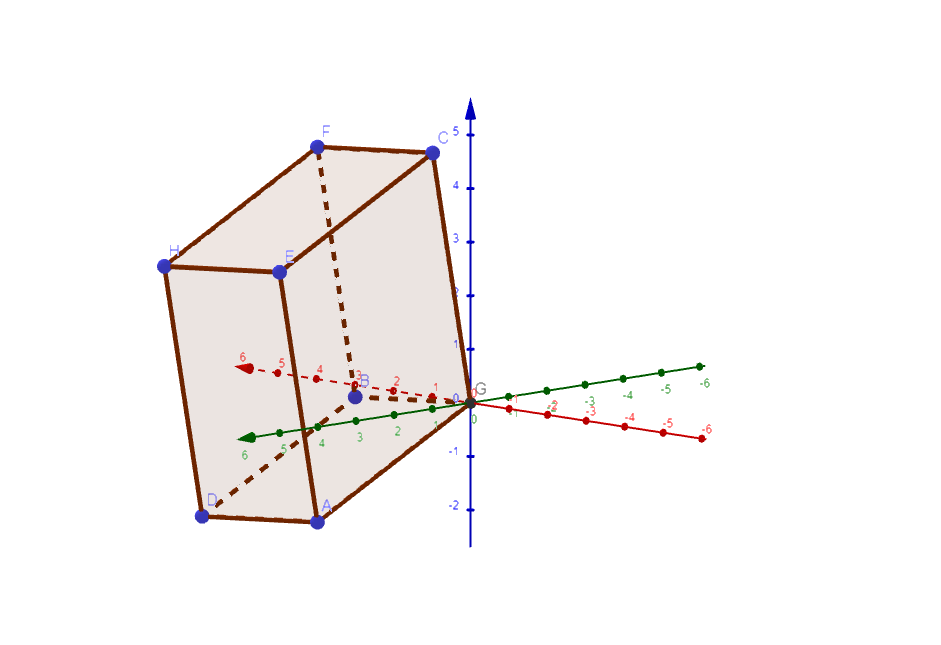
\includegraphics[width=\textwidth]{IntroductionCryptography/exercise-7-7.png}
		\caption{Exercise 7.7 - Fundamental domain of $L$}
	\end{figure}
	$\det (L) = \text{Vol} (\mathcal{F})$


7.43. $t = b_1 b_2 / \lVert b_1 \rVert^2$ and $b_2^* = b_2 - tb_1$ \\ $\Rightarrow b_2^* \cdot b_1 = b_1 (b_2 - tb_1) = b_1 b_2 - t \lVert b_1 \rVert^2 = b_1 b_2 - \frac{b_1 b_2}{\lVert b_1 \rVert^2} \cdot \lVert b_1 \rVert^2 = 0$ \\ Hence $b_2^* \perp b_1$ and $b_2^*$ is the projection of $b_2$ onto the orthogonal complement of $b_1$


7.44.
	
		 $\lVert a - tb \rVert^2 = (a - tb)^2 = a^2 - 2abt + t^2b^2 = \lVert a\rVert^2 + t^2 \lVert b\rVert^2 - 2abt \geq 0$ \\ $\Leftrightarrow a - tb = 0 \Rightarrow t = \frac{ab}{\lVert b \rVert^2}$
		 0
		 $(a - tb)\cdot b = ab - t \lVert b \rVert^2 = ab - \frac{ab}{\lVert b \rVert^2} \cdot \lVert b \rVert^2 = 0$. \\ Therefore $a - tb$ is the projection of $a$ onto the orthogonal complement of $b$
	
7.45.
	\begin{algorithm}[ht]
		\caption{Gauss's latice reduction algorithm}
		\begin{algorithmic}
			\While{True}
				\If{$\lVert v_2 \rVert < \lVert v_1 \rVert$}

				swap $v_1$ and $v_2$	
			
				$m \gets \lfloor v_1 \cdot v_2 / \lVert v_1 \rVert^2 \rceil$
			\EndIf
			\If{$m = 0$}

				return $(v_1, v_2)$
			\EndIf

			Replace $v_2$ with $v_2 - mv_1$
			\EndWhile
		\end{algorithmic}
	
	%\TitleOfAlgo{Gauss's latice reduction algorithm}
	\end{algorithm}
	
		 $v_1 = (14, -47)$, $v_2 = (-362, -131)$, 6 steps
		 $v_1 = (14, -47)$, $v_2 = (-362, -131)$, 6 steps
		 $v_1 = (147, 330)$, $v_2 = (690, -207)$, 7 steps
	


7.46.	
		 $W^\perp$ is the orthogonal complement of $W$ in $V$ $\Rightarrow \vec{z} \in W^\perp$, $\vec{z}\cdot\vec{y} = 0, \forall \vec{y} \in W$ \\ With $\vec{z_1}, \vec{z_2} \in W^\perp \Rightarrow \vec{z_1}\cdot\vec{y} = \vec{z_2}\cdot\vec{y} = 0, \forall \vec{y} \in W$ \\ $\Rightarrow (\vec{z_1} + \vec{z_2})\cdot\vec{y} = 0 \Rightarrow \vec{z_1} + \vec{z_2} \in W^\perp$ \\ $\alpha\vec{z_1}\cdot\vec{y} = \alpha \cdot 0 = 0 \Rightarrow \alpha\vec{z_1} \in W^\perp, \forall \alpha \in \mathbb{R}$
		 We have 2 methods
		
			 \textit{First method}: Show that $W \cup W^\perp = \{\vec{0}\}$. If $\vec{u}$ belongs to both $W$ and $W^\perp$, then $<u, u> = 0 \Rightarrow \vec{u} = \vec{0}$.
			
			Now denote $U = W + W^\perp$, we prove that $W = V$. We can choose an orthonormal basis in $U$ and extend it to orthonormal basis in $V$. Thus, if $U \neq V$, there is an element $\vec{e}$ in the basis of $V$ orthonormal to $U$. Since $U$ contains $W$, $e$ is orthonormal to $U \Rightarrow \vec{e} \in W^\perp$. The latter is a subspace of $W$, therefore $e$ is in $W$, which is contrary.
			 \textit{Second method}: Let $\{e_1, e_2, \cdots, e_k\}$ be an orthonormal basis of the subspace $W$. For each $v \in V$, let $$P(v) = \sum_{j=1}^{k} <v, e_j> e_j$$ $$\Rightarrow (\forall v \in V): v = \underbrace{P(v)}_{\in W} + \underbrace{(v - P(v))}_{\in W^\perp}$$
			The fact that $v - P(v) \in W^\perp$ is: 
			
			if $j \in \{1, 2, \cdots, k\}$ then 
			\begin{align*}
				<v-P(v), e_j> & = <v - \sum_{l=1}^{k}<v, e_l>e_l, e_j> \\
					& = <v, e_j> - <v, e_j> = 0	
			\end{align*}
			Since $\{e_1, \cdots, e_k\}$ is a basic of $W$, this prove that $v-P(v) \in W^\perp$
		
		 $\lVert v \rVert^2 = <v, v> = (aw + bw')^2 = a^2w^2 + 2abww' + b^2w'^2 = a^2 \lVert w \rVert^2 + 0 + b^2 \lVert w' \rVert^2 = a^2 \lVert w \rVert^2 + b^2 \lvert w' \rVert^2$
	
